\begin{figure*}[t]
\providecommand{\width}{}
\renewcommand{\width}{0.18\textwidth}
\centering
\begin{subfigure}[t]{\width}
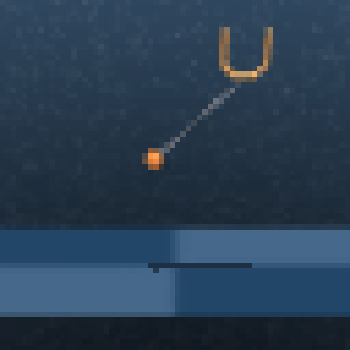
\includegraphics[width=\textwidth]{figures/tasks/cup}
\caption{Cup Catch}
\end{subfigure}\hfill%
\begin{subfigure}[t]{\width}
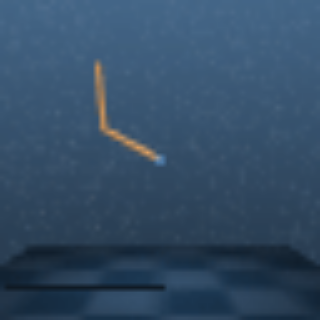
\includegraphics[width=\textwidth]{figures/tasks/acrobot}
\caption{Acrobot Swingup}
\end{subfigure}\hfill%
\begin{subfigure}[t]{\width}
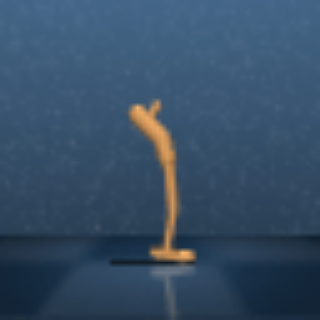
\includegraphics[width=\textwidth]{figures/tasks/hopper}
\caption{Hopper}
\end{subfigure}\hfill%
\begin{subfigure}[t]{\width}
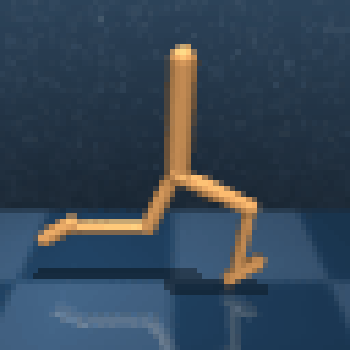
\includegraphics[width=\textwidth]{figures/tasks/walker}
\caption{Walker}
\end{subfigure}\hfill%
\begin{subfigure}[t]{\width}
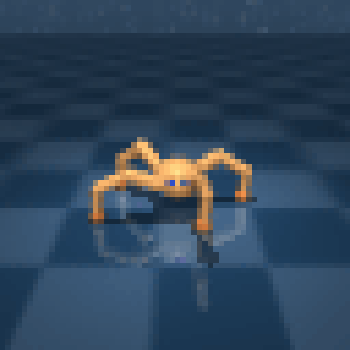
\includegraphics[width=\textwidth]{figures/tasks/quadruped}
\caption{Quadruped}
\end{subfigure}\hfill%
\caption{我们实验使用的 20 个视觉控制任务中，图中展示了其中 5 个任务的图像观测。这些任务覆盖多种挑战，包括接触动力学、弱奖励、多自由度控制和 3D 环境。此前部分任务尚未被世界模型方法解决。}
\label{fig:tasks}
\vspace*{-1ex}
\end{figure*}
